%\section{Company-wide}
\section{Organization and employees}
\label{sec:companywide}

The company is divided into two departments, Product \& Sales (P\&S) and Research \& Development (R\&D). The focus of the P\&S department is mainly customer contact, requirements, and testing. The R\&D department mainly focuses on topics regarding design and implementation. From these teams, we have created cross-functional teams with specific tasks. These teams have developed during the project to focus on different tasks as the project's needs have changed, see more under \ref{sec:companywide:subsection:cft} %expand this part 
\subsection{Roles}
\begin{figure}[ht]
    \centering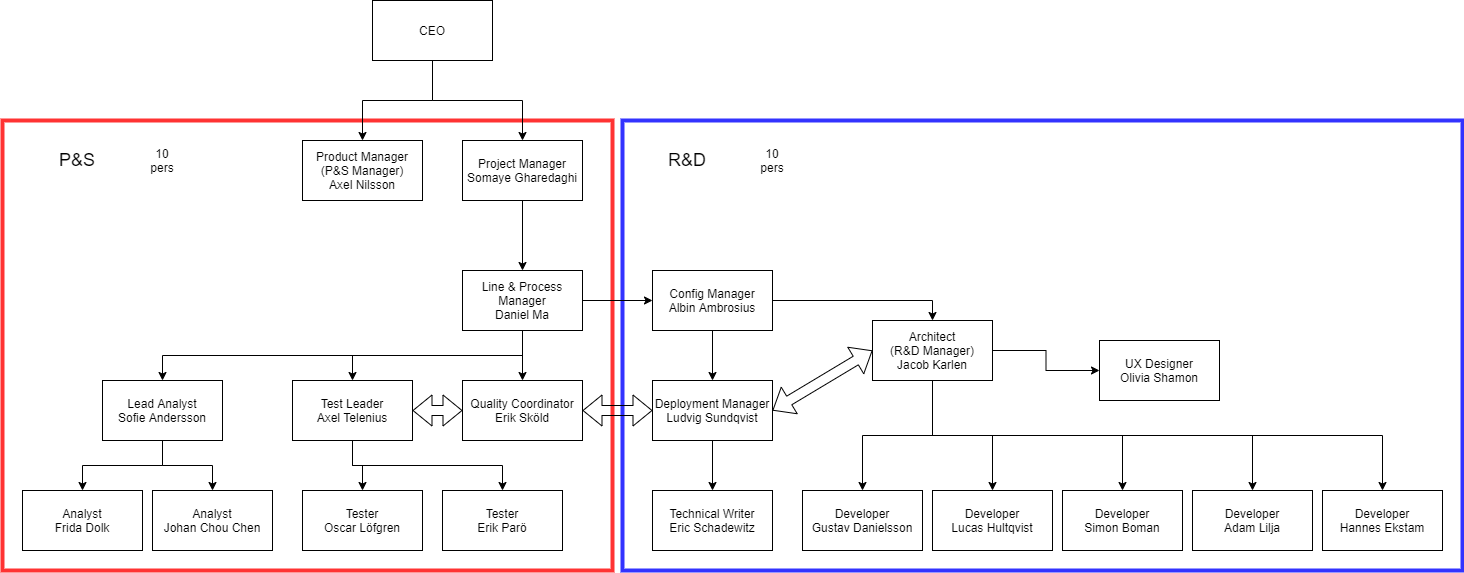
\includegraphics[width=1 \linewidth]{figures/company flowchart.png}
    \caption{Company Flowchart}
    \label{fig:example2}
\end{figure}


%description of each role in details from teams and their names
\subsubsection*{Product Manager – Axel Nilsson}
A strategic product owner is a link between the customer and the developers. This means handling the product backlog and prioritizing requirements in the best way possible to match customer needs. Also, creating a vision for the product so the whole team knows what we are working towards. 

\subsubsection*{Project Manager – Somaye Gharedaghi} 
Breaking down the work by creating the project plan, making sure that everyone has something to do in a timely manner, making sure that everyone has the view of the plan to know how they can contribute and collaborate, running the meetings, and keeping the project organized. These all are achievable through regular managers meetings or one by one, keeping in touch with managers, listening to their concerns, and setting agenda for meetings according to following up the progress of the project and managers' concerns. As well as presenting the weekly report to the CEO at CEO Meeting and sending weekly status reports to the CEO, the consulting supervisors, the examiner, and the company's employees. 

\subsubsection*{Line \& Process Manager – Daniel Ma}
Ensures suitable working environments and sees that everyone feels involved and content. Handles formal communication with the company leadership. Develops and handles the company's processes along with the Quality coordinator.

\subsubsection*{Lead Analyst - Sofie Andersson} 
The main responsibility is to contact our customer and understand what they want from our system and what they need. Also responsible for making progress in the analyst work and communicating to the manager group about it. 

The analyst team is responsible for defining requirements and user stories so that the development group knows what to do and has customer meetings.  

\subsubsection*{Analysts - Frida Dolk \& Johan Chou Chen} 
Analysts are responsible with the Lead analyst to structure the work with the customer and align the customer needs with the rest of the company. Shall understand customer's desires and put these into requirements in a concrete, detailed and organized way and deliver to the developer team. 

\subsubsection*{Test Leader - Axel Telenius} 
Handling testing operations towards the customer, following up work by the test team, and coordinating with the quality coordinator to ensure software meets specifications from the testing point of view.

\subsubsection*{Testers - Oscar Löfgren \& Erik Parö}
Testers assist the test leader with the test, assist the test leader with coming up with a clear plan for the testing, and report the test results. They are responsible for creating relevant test documents and making sure to follow them. 

\subsubsection*{Quality Coordinator - Erik Sköld} 
Measures and monitors the product quality and initiates necessary changes of product and process. Responsible for the explicated plan for quality assurance. Works together with the testing team on the software quality assurance plan. Reviews decisions on code conventions, test tools, and reporting. Collects means of quality work, verifies traceability, and makes sure the work fits together. 

\subsubsection*{Configuration Manager – Albin Ambrosius} 
Ensures that all tools, software or hardware, are being utilized and progress is being tracked. This role will see that everyone is notified of changes in the tools or assets that we create.  Handles the set-ups for new tools and communicates with both the development team and company leadership through R\&D reports.  

\subsubsection*{Architect – Jacob Karlén} 
Specifies and decides on high-level architecture, target environment, and components to be used. Ensures that functional and non-functional requirements are met and coordinates with other teams on technical matters. Responsible for the Architecture Notebook.  

\subsubsection*{R\&D Manager – Ludvig Sundqvist}
Responsible for scheduling, sending out agendas and moderating R\&D meetings an,d coordinating the work within the department.  

\subsubsection*{UX Designer – Olivia Shamon} 
Specializes in setting targets and realizing the user experience of the system. Creates prototypes of the system for the developers.  

\subsubsection*{Deployment Manager – Ludvig Sundqvist}
Makes sure the product is made available to the customer and plan and prepare for continuous deployment. Works as a middleman between the testers and developers works closely with the architect and test leader. This role is the responsible manager for Docker, GitLab, and containers. 

\subsubsection*{Technical Writer – Eric Schadewitz} 
Ensures that the output of the project is accessible to our customer. Produces instructions on how to use the system the way it was developed to be used. Also documents suggestions for further development. 

\subsubsection*{Developers – Gustav Danielsson, Lucas Hultqvist, Simon Boman, Adam Lilja \& Hannes Ekstam Ljusegren} 
Have the main responsibility of realizing requirements into functions of the software solution. 

\subsection{Cross-functional teams}
\label{sec:companywide:subsection:cft}
The company is further divided into three cross-functional teams (hereinafter CFT), with members from both departments and with different roles. See appendix \ref{sec:CFTs-appendix} for the team structures. The idea with the CFTs is to speed up development by ensuring that the right competence is present in each team and that a wide range of competencies is present. One key area of the project is the requirement specification. The company's analysts carry the expertise of this area, and thus a decision was made to have one analyst in each CFT so that this knowledge is dispersed throughout the whole company. The members and structures of the CFTs may change during the development phase (between iterations) depending on customer needs, course requirements, or any other reasonable reason.

For each iteration, each CFT shall have different responsibilities as planned by the managers. During the pre-study, each CFT shall develop a unique prototype to showcase to the customer. One prototype shall be chosen from the customer feedback, and this prototype shall be the basis for the development. In the first iteration, one team develops the software's back-end, and two teams focus on the front-end (software overview and patient journal, respectively). In the second iteration, the back-end team shall swap focus to front-end development if back-end development is finished. 

To address slow development progress and isolated developers and testers (feedback received from, e.g., complaints, retrospectives, and company surveys), the CFTs are restructured for iterations three and four. During these iterations, the CFTs have the following focus areas: CFT1 shall be developer-heavy and focus on completing the issues with the highest rank; CFT2 shall focus on UX design, provide the development team with prototypes when needed and also test the implemented component to verify that they work in the intended way UX-wise; CFT3 shall focus on testing and quality, with tasks such as implementing a pipeline in GitLab with automated tests and accepting merge-requests. 